% Chapter 2: Background and Related Work
Understanding the methodology behind this thesis requires first examining how Transformer architectures and Language Models have evolved. This chapter explores that evolution and briefly introduces the LLaMA family as it will be relevant to this project in (see Chapter \ref{chap:methodology}). The discussion then turns to the hardware limitations which influenced design decisions in this context. Finally, the chapter reviews research and literature on LLM optimization techniques relevant to this work.

\section{Early Language Models}
Before the emergence of the Transformer architecture, language models predominantly relied on \textit{Recurrent Neural Networks} (RNNs). These networks represent an evolution of the \textit{Multi-Layer Perceptron} (MLP), and incorporate cyclic connections within their architecture to create recurrent circuits. Such design enables the model to maintain a form of memory, allowing it to consider previous inputs when generating predictions and thereby capturing long-range dependencies inherent in sequential data such as text.

Despite their theoretical advantages, RNNs suffer from a critical limitation known as the vanishing gradient problem \cite{rnn}. During backpropagation, gradients from earlier time steps decay exponentially as they flow backward through the network layers. This degradation severely hampers the network's ability to be trained effectively, as the influence of distant past information becomes negligible in the parameter updates.

To address these limitations, Hochreiter and Schmidhuber introduced \textit{Long Short-Term Memory} (LSTM) networks \cite{lstm} \cite{hinton-lstm}, which revolutionized sequence modeling through their sophisticated gating mechanisms. LSTMs employ specialized memory cells designed to selectively retain, update, and output information across extended sequences.  The architecture incorporates three fundamental gate types that regulate information flow:
\begin{itemize}
    \item The \textit{input gate} determines the extent to which new information from the current input should be incorporated into the cell state. It evaluates the relevance of incoming data and controls its integration with existing memory.
    \item The \textit{forget gate} governs the retention of information from previous time steps, deciding which aspects of the historical cell state remain relevant and should be preserved.
    \item Finally, the \textit{output gate} regulates how much of the current cell state should be exposed to subsequent layers, effectively controlling what information propagates forward in the network.
\end{itemize}

All of these gates can be clearly observed in Figure \ref{fig:lstm-architecture}. This gating mechanism allows LSTMs to maintain gradient flow over much longer sequences compared to vanilla RNNs. Thus, they can capture dependencies spanning hundreds of time steps, making them particularly effective for tasks requiring long-term context understanding such as language modeling, machine translation, and text summarization.
\begin{figure}[!htbp]
\centering
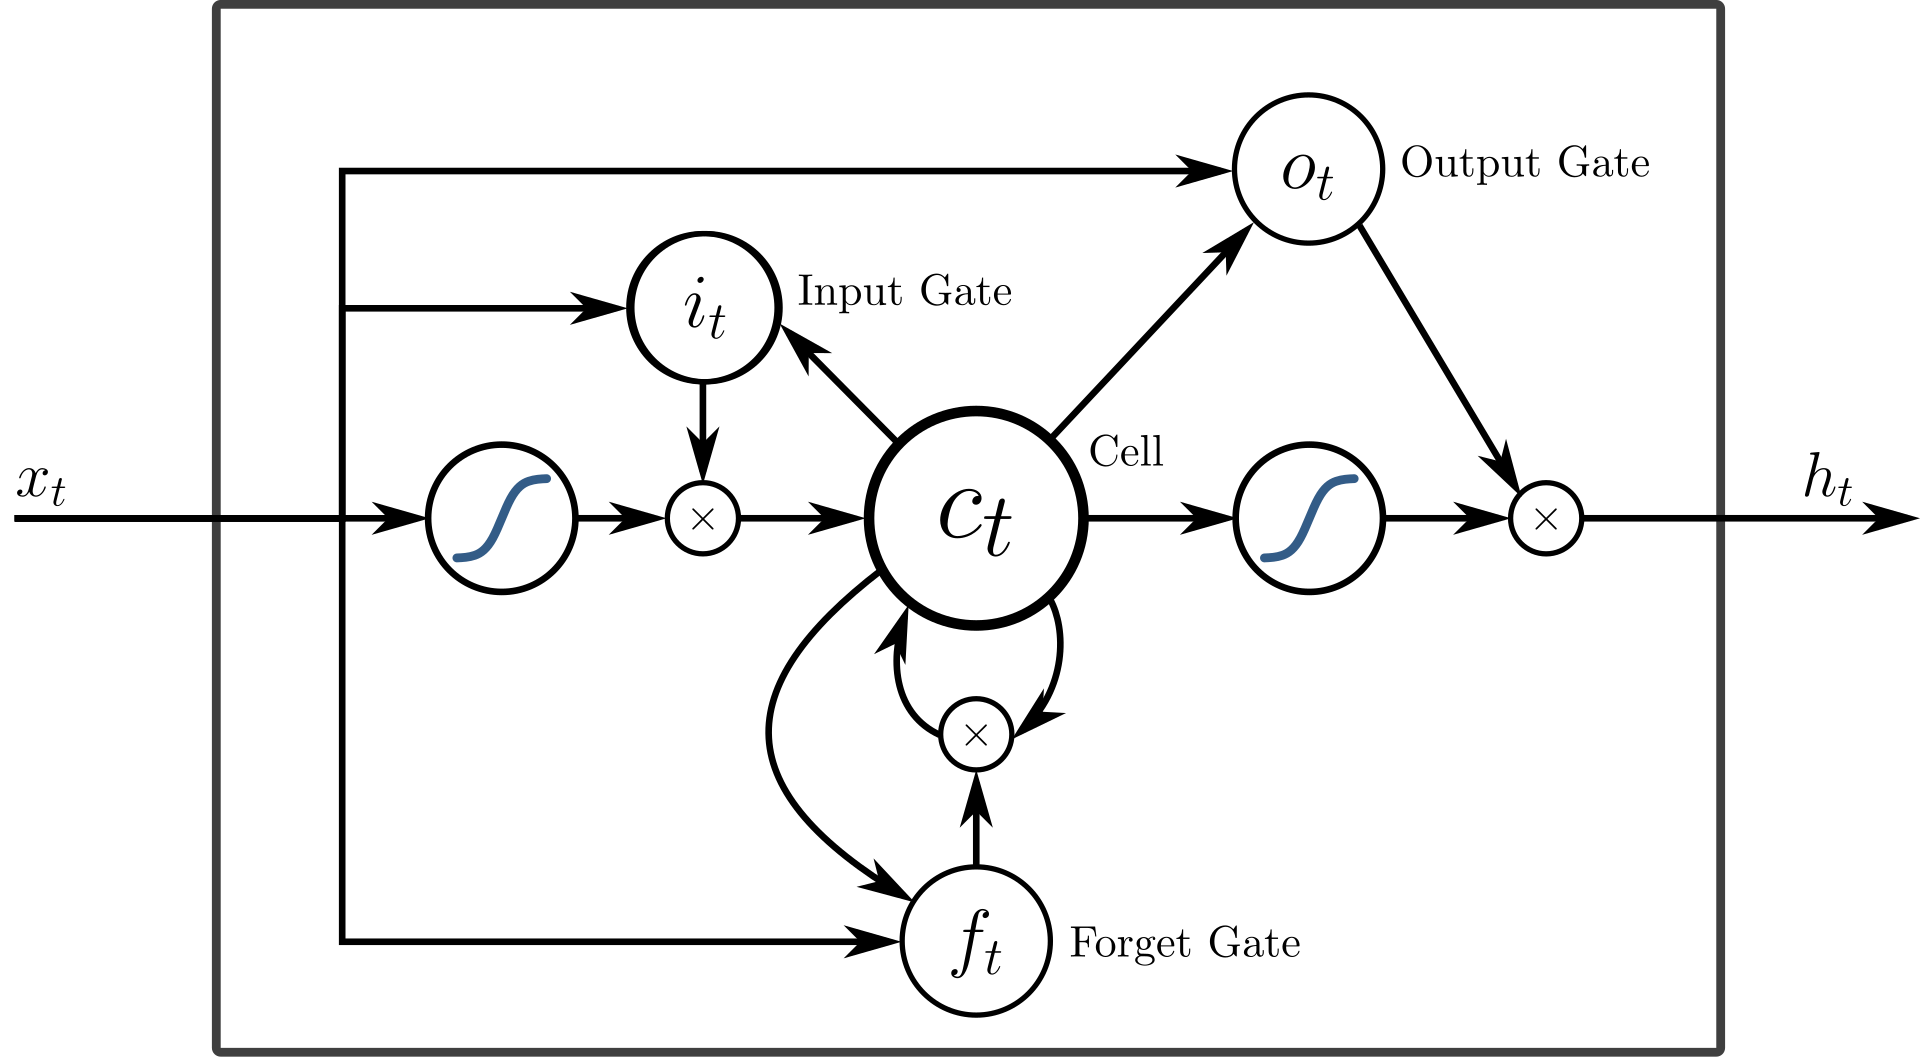
\includegraphics[width=0.7\textwidth]{image.png}
\caption[LSTM cell architecture]{Architecture of an LSTM cell showing the three gating mechanisms. The input gate (left) controls information incorporation, the forget gate (center) manages memory retention, and the output gate (right) regulates information flow to subsequent layers. The cell state (horizontal line) maintains long-term memory throughout the sequence. The image was retrieved from \cite{hinton-lstm}.}
\label{fig:lstm-architecture}
\end{figure}

While LSTMs significantly improved the ability to model sequential data, they still faced challenges in terms of parallelization and context understanding, especially when compared to Transformers.  Nevertheless, LSTMs are still widely used for various \textit{natural language processing} (NLP) tasks, including text generation \cite{lstm_textgeneration}.

\section{The Transformer Architecture}  \label{transformer_architecture}

The Transformer architecture, introduced by Vaswani et al. \cite{attention_is_all_you_need}, fundamentally changed how we approach sequence modeling by abandoning recurrent connections entirely in favor of attention mechanisms. Unlike LSTMs that process sequences step-by-step, the Transformer can examine all positions simultaneously, and as such it can be easily parallelized during training. Moreover, it can capture long-range dependencies thanks to the attention mechanism.

\subsection{The Attention Mechanisms}

At the core of the Transformer lies the attention mechanism, which addresses the information bottleneck created when sequence models compress an entire input sequence into a single fixed-size vector. This bottleneck becomes particularly problematic for long sequences, where important information can be lost or diluted.

Attention allows a model to dynamically focus on different parts of the input sequence when generating each output token, similar to how humans selectively concentrate on relevant information when reading a book. This is done, essentially, by directly comparing and relating any two positions in a sequence, regardless of their distance (i.e. self-attention).

\subsection{Scaled Dot-Product Attention}

The attention mechanism is computed using three matrices derived from the input:

\begin{equation}
\text{Attention}(Q, K, V) = \text{softmax}\left(\frac{QK^T}{\sqrt{d_k}}\right)V
\end{equation}

Each component serves a specific purpose:

\begin{itemize}
   \item \textbf{Queries (Q)}: Generated by $Q = XW_Q$ where $X$ is the input and $W_Q \in \mathbb{R}^{d_{\text{model}} \times d_k}$. Each query vector can be seen as asking ``what information am I looking for?''
   \item \textbf{Keys (K)}: Generated by $K = XW_K$ where $W_K \in \mathbb{R}^{d_{\text{model}} \times d_k}$. Keys act as indexed labels for each position's content.
   \item \textbf{Values (V)}: Generated by $V = XW_V$ where $W_V \in \mathbb{R}^{d_{\text{model}} \times d_v}$. Values contain the actual information to be retrieved.
\end{itemize}

The attention computation proceeds in four steps:

\begin{enumerate}
   \item \textbf{Similarity Computation}: $QK^T$ produces a $n \times n$ matrix where entry $(i,j)$ represents how much position $i$ should attend to position $j$. The dot product naturally measures similarity between query and key vectors.

   \item \textbf{Scaling}: Division by $\sqrt{d_k}$ (where $d_k$ is the dimensionality of the keys) prevents the dot products from becoming too large. Without scaling, large dot products push the softmax function into regions with extremely small gradients. For example, if $d_k = 512$, dot products could reach magnitudes of $\pm 20$ or more, causing softmax to output distributions close to one-hot vectors.

   \item \textbf{Normalization}: The softmax function converts similarity scores into a probability distribution: $\text{softmax}(x_i) = \frac{e^{x_i}}{\sum_{j=1}^n e^{x_j}}$. This ensures attention weights sum to 1 and creates a differentiable selection mechanism.

   \item \textbf{Weighted Aggregation}: The attention weights are applied to the value vectors, producing a weighted sum that represents the attended information for each position.
\end{enumerate}

\subsection{Multi-Head Attention}

The Transformer employs multi-head attention so that each head can focus on different parts of the input. Some heads might track syntax, others semantics, positions, etc. This is done by projecting the input matrices $Q, K, V$ by $h$ times using different learned linear projections:
\begin{equation}
(QW_i^Q, KW_i^K, VW_i^V)
\end{equation}
Given this, each head is computed as:
\begin{equation}
\text{head}_i = \text{Attention}(QW_i^Q, KW_i^K, VW_i^V)
\end{equation}
As such, the final equation for multi-head attention is:
\begin{equation}
\text{MultiHead}(Q, K, V) = \text{Concat}(\text{head}_1, \ldots, \text{head}_h)W^O
\end{equation}

Each head uses different projection matrices $W_i^Q \in \mathbb{R}^{d_{\text{model}} \times d_k}$, $W_i^K \in \mathbb{R}^{d_{\text{model}} \times d_k}$, and $W_i^V \in \mathbb{R}^{d_{\text{model}} \times d_v}$, where typically $d_k = d_v = d_{\text{model}}/h$ for $h$ heads. 

Multi-head attention essentially gives the model multiple different perspective of the same input, and it is a vital system that contributes to make this architecture so powerful.

\subsection{Positional Encodings}

Since attention is permutation-invariant, the Transformer requires explicit positional information. The original work uses sinusoidal positional encodings:

\begin{align}
PE_{(\text{pos}, 2i)} &= \sin(\text{pos}/10000^{2i/d_{\text{model}}}) \\
PE_{(\text{pos}, 2i+1)} &= \cos(\text{pos}/10000^{2i/d_{\text{model}}})
\end{align}

These encodings have useful properties: they create unique representations for each position, allow the model to learn relative positions through linear combinations, and can theoretically handle sequences longer than those seen during training.

\subsection{Encoder-Decoder Transformers}

Transformer-based models generate text by predicting the next token in a sequence, conditioned either on an external input (encoder-decoder models) or on the sequence generated so far (decoder-only models). The former is what the original Transformer architecture~\cite{attention_is_all_you_need} follows.

\begin{itemize}
  \item The \textbf{encoder} processes the full input sequence in parallel, producing a series of contextual embeddings that capture the meaning and structure of the input tokens.
  \item The \textbf{decoder} generates the output sequence token by token, using the embeddings from the encoder.
\end{itemize}

This design enables the model to generate outputs that are grounded in the input sequence, rather than generating new text from scratch. Thus, such design is well-suited for sequence-to-sequence tasks such as machine translation.

\subsection{Decoder-Only Transformers}

In decoder-only Transformers, there is no separate encoder module. The model predicts each token based only on the previously generated tokens, modeling the joint distribution \( p(x_1, x_2, \ldots, x_n) \) autoregressively. This means that the model outputs one token at a time, appends it to the input, and repeats until a stopping condition is met.

These architectures are simpler and more scalable, and they are the ones employed in large language models such as GPT \cite{gpt} and, of course, LLaMA \cite{llama}.

Decoder-only Transformers are ideal for open-ended text generation and other tasks where the output is not conditioned on a separate input sequence.
Figure \ref{fig:sidebyside} shows a comparison of encoder-decoder and decoder-only transformer architectures.

\section{A Brief Overview on the LLaMA Family of Models} \label{llama_overview}

The \textit{Large Language Model Meta AI} (LLaMA) family~\cite{llama}, developed by Meta AI, comprises a series of transformer-based autoregressive language models designed as competitors to OpenAI's GPT model family. The original LLaMA models were introduced in early 2023, followed by LLaMA 2 \cite{llama2} later that year and LLaMA 3 \cite{llama3} in 2024.

The models vary in the number of parameters and capabilities, with the newer versions offering improved performance over the older ones. In particular, with LLaMA 3, Meta introduced models ranging from 8B to 405B parameters with major upgrades in both training scale and performance over LLaMA 2, while approaching results to OpenAI's GPT-4 \cite{gpt4} \cite{llama3}.

The main feature of LLaMA, however, is its open-weight release strategy. Unlike most proprietary models, Meta provides access to the model weights under a research-friendly license, enabling the broader research community and industry practitioners to experiment with, fine-tune, and deploy large-scale language models without relying on closed systems. This openness has led to a proliferation of derivative models, and thus to the making of the project central to this thesis.


\begin{figure}[htbp]
    \centering
    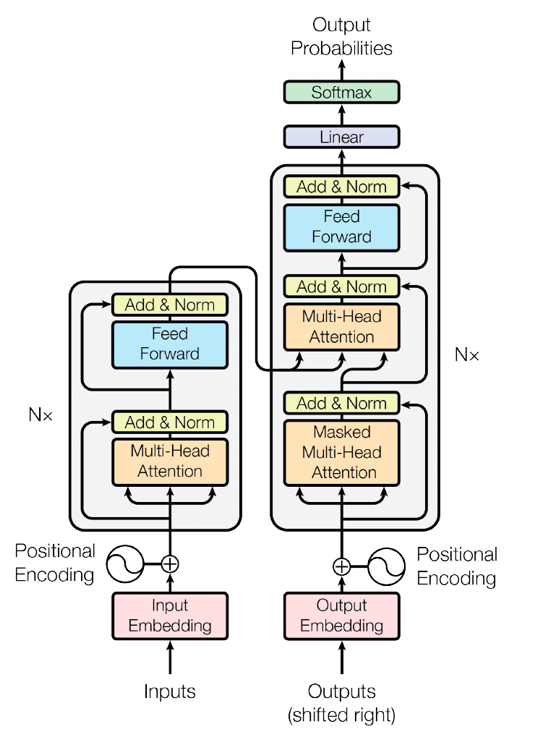
\includegraphics[width=0.45\textwidth]{transformer.png}
    \hfill
    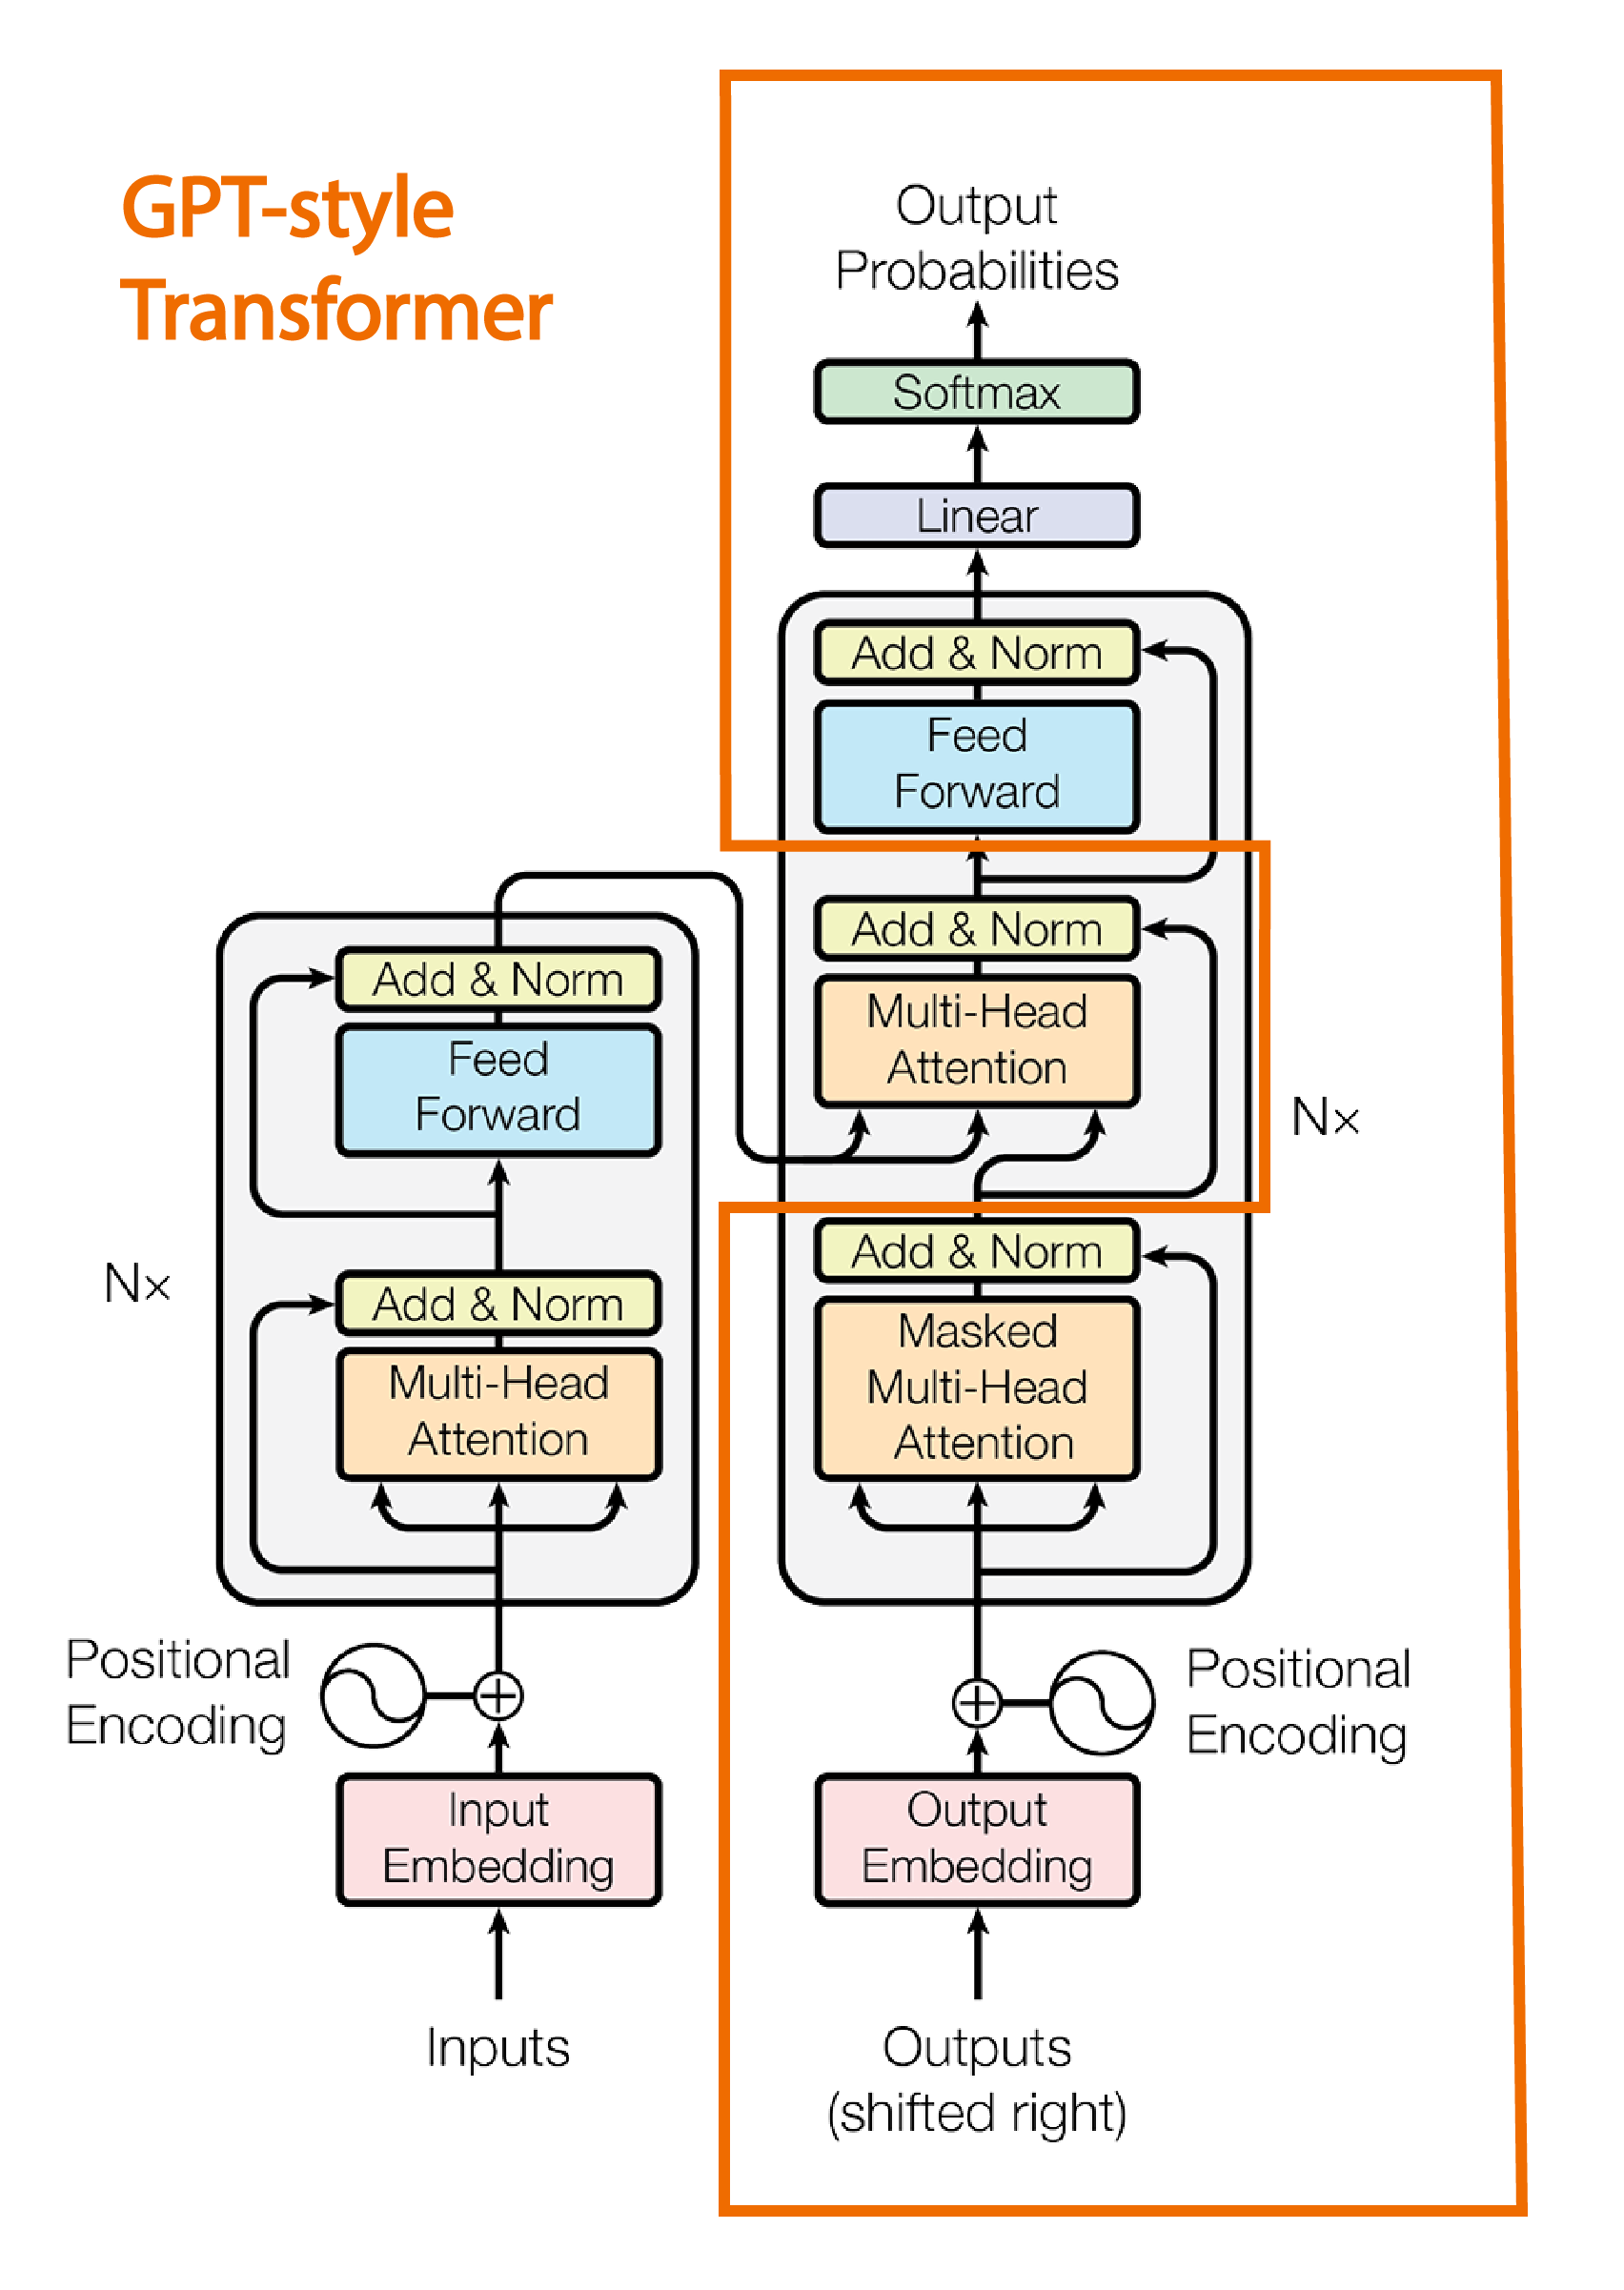
\includegraphics[width=0.45\textwidth]{transformer-gpt.png}
    \caption[Transformer architectures comparison]{On the left, a standard Transformer architecture, which consists of an encoder and a decoder. On the right, we can observe the same architecture, while highlighting the only the layers used by a GPT-style model, which is a decoder-only transformer. The main difference is that the decoder does not attend to the encoder's output, allowing for auto-regressive generation. The image is a modified version of the one found on Vaswani et al. research paper \cite{attention_is_all_you_need}.}
    \label{fig:sidebyside}
\end{figure}

\section{A Look at the Target Hardware} \label{target_hardware}

The hardware constraints of an ideal target deployment scenario provide an additional compelling motivation for this compression work, beyond the environmental and social concerns outlined in Chapter 1. The envisioned platform is Siracusa \cite{target_hardware}, a heterogeneous RISC-V \textit{System-on-Chip} (SoC) fabricated in 16 nm CMOS technology, which exemplifies the stringent resource constraints typical of edge XR devices designed for \textit{Extended Reality} (XR) applications. While this project does not involve actual deployment or testing on this specific hardware, the severe memory limitations and computational constraints characteristic of such platforms make LLM compression not merely an environmental imperative, but a fundamental requirement for any practical edge deployment. A visual representation of Siracusa's architecture can be found in Figure \ref{fig:siracusa}.

Siracusa's memory hierarchy presents the primary constraint for the optimization efforts. The system features a three-tier memory organization: 256 KiB of L1 \textit{Tightly-Coupled Data Memory} (TCDM) SRAM organized into 16 word-interleaved banks, 4 MiB of SRAM tile memory, and 4 MiB of \textit{magnetoresistive memory} (MRAM) for weight storage, totaling 8.5 MiB. The memory hierarchy uses specialized allocation: MRAM stores weights while tile memory handles activations. However, it may be obvious to the reader that this amount of storage is rather limiting: exceeding the 4 MiB weight memory capacity forces reliance on slower off-chip transfers that can increase inference latency by orders of magnitude.

The computational architecture features an octa-core RISC-V cluster paired with the N-EUREKA neural processing engine, which provides substantial parallel processing capability with peak performance reaching 1.95 TOp/s. However, this performance is only achievable when models fit entirely within the on-chip memory hierarchy. The 92 Gbit/s bandwidth between MRAM and the neural engine enables efficient weight streaming, but only when the model's memory footprint aligns with the available storage capacity.

\begin{figure}[htbp]
    \centering
    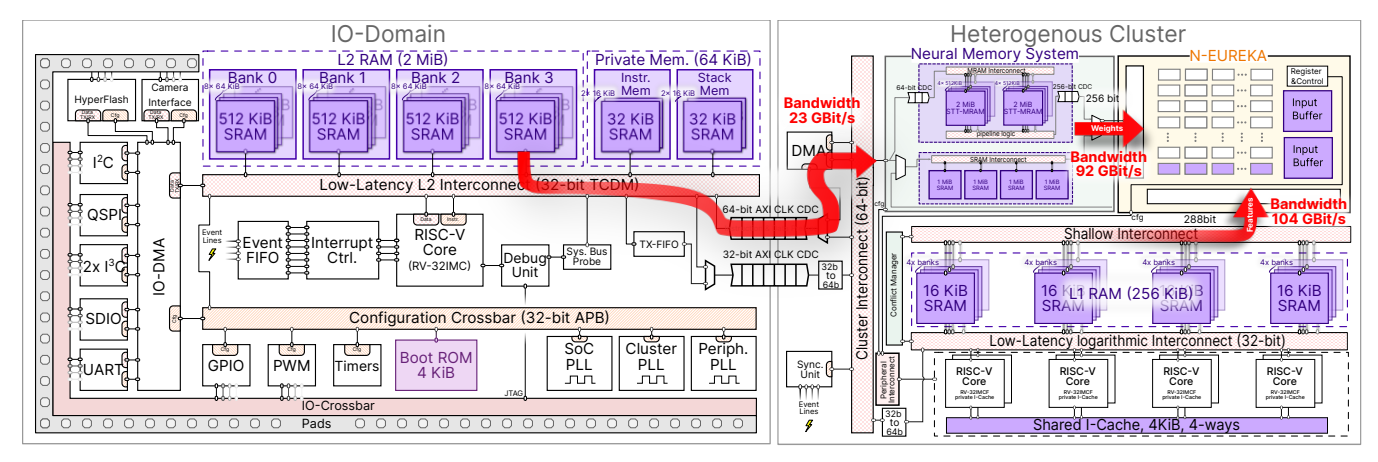
\includegraphics[width=1\textwidth]{siracusa.png}
    \caption[The architecture of Siracusa]{A visual representation of Siracusa's architecture. On the upper right we can see the N-EUREKA accelerator, while on the lower right the RISC-V cluster is visible. This image was sourced from the original paper \cite{target_hardware}.}
    \label{fig:siracusa}
\end{figure}

These specifications illustrate the type of resource constraints that drive the need for aggressive compression techniques in edge AI deployment scenarios, and the compression pipeline developed in this work represents a promising approach toward achieving the level of optimization required for practical deployment on such platforms.
\section{Related Work}

This section examines some techniques that have proven effective for compressing large language models, providing an overview of the current available research and inspiration for novel methods that could extend the project's scope (further explored in Section \ref{future_work}).

\subsection{Knowledge Distillation} \label{distillation_paragraph}

Knowledge distillation \cite{distillation} has emerged as a fundamental technique for compressing pre-trained language models by transferring knowledge from a large "teacher" model to a smaller "student" model. In particular, the core principle involves training the student to match not only the ground truth labels but also the soft predictions of the teacher model, in order to capture richer information about the decision boundaries learned by the larger network.

Traditional distillation approaches can be categorized into task-specific and task-agnostic variants. Task-specific distillation first fine-tunes the teacher model on a particular downstream task before distillation, while task-agnostic distillation maintains a general-purpose student that can be efficiently adapted to various tasks.

A significant challenge in conventional distillation arises from the substantial capacity gap between teacher and student models. When the student model has significantly fewer parameters than the teacher, the prediction discrepancy can become too large for effective knowledge transfer, particularly over massive amounts of open-domain training data. This limitation has motivated more sophisticated initialization and training strategies.

\textit{Homotopic Distillation} (HomoDistil) \cite{homodistil} addresses this challenge through an innovative approach that combines iterative pruning with distillation. Rather than initializing a small student model from scratch, HomoDistil begins with the full teacher model and gradually prunes neurons while simultaneously distilling knowledge. This maintains a small prediction discrepancy throughout training, ensuring effective knowledge transfer even at high compression ratios.

The key insight of HomoDistil is that starting from the teacher model and iteratively removing the least important components prevents the dramatic performance drops typically seen with aggressive compression. At each training iteration, the method computes importance scores for individual neurons and removes those with minimal impact on the loss function. This pruning strategy is very similar to one adopted in this document for removing whole layers (i.e. depth pruning), as shown in Section \ref{depth_pruning}. This gradual reduction maintains network connectivity and allows the distillation loss to effectively guide the compression process.

\subsection{Pruning Approaches}

As detailed in Chapter \ref{chap:methodology}, pruning significantly reduces model complexity through two main approaches. Width pruning targets individual neurons or layers (usually) within a transformer block, while depth pruning eliminates entire submodules.

In a similar way to this project, \textit{Two-Stage Structured Pruning} (2SSP) \cite{2ssp} combines these approaches optimally. This method applies width pruning to feed-forward networks in the first stage, followed by depth pruning of attention modules in the second stage.

For width-pruning, importance scores are computed based on the magnitude of neuron activations across calibration samples, which are then used to remove entire neurons. On the other hand, the second stage targets attention modules which are iteratively removed based on their impact on model perplexity. This coarser-grained approach proves effective because attention modules often exhibit high redundancy.

A critical innovation in 2SSP is the automatic balancing of sparsity between the two stages. The method uses an adaptive formula that considers the relative sizes of feed-forward and attention components to determine optimal allocation of parameter reduction across stages. This ensures that neither component becomes a bottleneck while maintaining overall performance.

While some similarities can be found, this work differs from the pruning approach adopted in this project in two fundamental ways.
\begin{itemize}
\item While we target attention weight matrices for width-pruning, their method focuses on FFN components. In addition, the structured width-pruning strategies are entirely distinct: 2SSP removes complete rows and columns by slicing weight matrices rather than using a ratio-based structural pruning (see Section \ref{wanda}).
\item Our method for computing layer importance during depth-pruning employs a compound metric rather than relying solely on perplexity-based measures (see Section \ref{depth_pruning}).
\end{itemize}.

Another promising approach to structured pruning is demonstrated by \textit{Sheared LLaMA} \cite{sheared_llama}, which takes a fundamentally different perspective by viewing pruning as an initialization step rather than a final compression technique. This method employs targeted structured pruning to compress LLaMA2-7B down to 1.3B and 2.7B parameter models, followed by substantial continued pre-training to recover performance.

In particular, Sheared LLaMA combines two techniques: first, a constrained optimization approach that prunes models to precisely match target architectures (derived from existing well-optimized models), and second, dynamic batch loading that adjusts training data composition based on domain-specific loss recovery rates. This addresses a critical observation that pruned models retain different levels of knowledge across domains (e.g. maintaining better performance on code repositories while losing more capability on natural language text).


